\documentclass{article}
\usepackage[hidelinks]{hyperref}
\usepackage{graphicx}    
\usepackage{wrapfig}
\usepackage{amsmath}
\usepackage{amssymb}
\newcommand\R{{\mathbb R} }
\renewcommand\S{{\mathcal S}}
\newcommand\goesto{{\longrightarrow}}

\begin{document}
\title{Transformation of a bivariate $\Gamma$-distribution}
\date{2020-02-04}

\author{Paul Libbrecht, IUBH Advanced Statistics, \href{https://creativecommons.org/licenses/by/4.0/}{CC-BY}}
\maketitle



% =================================================

\section{Statement}

Let $X$ and $Y$ be independent random variables $\sim\Gamma(2,5)$; we call $f_X$ and $f_Y$ their density function.
Compute the density function of the variable $T=X+Y$.

\section{Straight of the theory}

$X$ and $Y$ are random variables, that is they are $X:\S \longrightarrow \R^+$ and $Y:{\S }\longrightarrow \R^+$.
They are Gamma variables of parameters $\alpha=2$ and $\beta=5$ (see \cite{Wikipedia-Gamma}), thus, they are distributed in such a way that given a set of real-numbers $E$:

$$P(Y\in E) = P(X\in E) 
  = \int_{t\in E} \frac{\beta^\alpha}{\Gamma({\alpha})}t^{\alpha-1}e^{-\beta t}dt 
  = \int_{t\in E} \frac{5^2}{1} t e^{-5t}dt 
  = \int_{t\in E}25te^{-5t}dt$$
  
Let us call $f_X(t)=f_Y(t) = 25te^{-5t}$.

% ===================================================
\section{Transformations?}



Given a multivariate continuous random variable $X: {\S } \rightarrow D$ (having values in any set) and a mapping $g: D \rightarrow E$ a mapping, the {\bf transformed random variable} $g \circ X$, often written as $g(X)$ is defined by $g(X)(s) = g(X(s))$.  

We assume $E,D\subset \R^n$. Then this is the same as saying: given a series of random variables $X_i: \S \goesto \R$ where $0\le i \le n$ and $(X_1, \dots, X_n) \in D$ and a series of functions $g_i: \R^n \goesto \R$ where $(g_1(x_1,\dots,x_n), \dots, g_n(x_1,\dots,x_n))\in E$ when $(x_1,\dots, x_n)\in E$.

Suppose that $D$ and $E$ are subsets of $\R^n$ and that $g$ is a derivable tranformation (which means: $g_i(x_1,...,x_n)$ is derivable, i.e. $\frac{\partial g_i}{\partial x_j}$ exists for each $0 \le i,j  \le n$).  

The transformation theorem, proved in \cite[2.7]{Hogg-McKean}, says that:

\begin{itemize}
\item $g(X)$ It is a continuous random variable.
\item if $D, E \subset \R ^n$ and $X$ is a continuous random variable with pdf $f_X:D \rightarrow \R $ then the pdf of
  $g(X)$, noted $f_{g(X)}$, is equal to the following, $\forall {\mathbf a} \in E$:
\end{itemize}

$$  f_{g(x)}({\mathbf a}) = f_X(g^{-1}({\mathbf a})) \cdot | J_{g^{-1}}({\mathbf a})|$$

It is important to note that $D$ and $E$ are rarely equal to complete $\R^n$. E.g. It could be a subset of a plane where the lowest $x$ depends on $y$.

% ===================================================
\section{Calculation with a transformation}

Introduce the transformation 

\begin{alignat*}{2}
g:\quad & \R^+ \times \R^+ &\longrightarrow \quad & O \\
& (x,y) & \mapsto\quad & (a,b) = g(x,y) = (x+y, x-y) 
\end{alignat*}

\begin{wrapfigure}{r}{32mm}\includegraphics[width=30mm]{transformation-domain}\vspace{10mm}\end{wrapfigure}
This transformation is  a bijection if $O$ is:

$$O = \{ (a,b)\in\R^2 \mid a+b \geq 0 \mbox{ and } a-b\geq 0\}$$

Its inverse is:

$$ g^{-1}: O \longrightarrow \R^+ \times \R^+$$
$$ (a,b) \mapsto (x,y) = g^{-1}(a,b) = \left( \frac{1}{2} (a+b), \frac{1}{2}(a-b) \right)$$

because $g^{-1} (g(x,y)) = g^{-1}(x+y, x-y) = \left ( \frac{1}{2} (x+y+x-y), \frac{1}{2} ( x+y-x+y) \right ) = \left ( \frac{1}{2} 2x, \frac{1}{2} 2y\right ) = (x,y)$


We apply the multivariate transformation theorem (\cite[2.7]{Hogg-McKean}) and thus compute the Jacobian:

\newcommand{\half}{\frac{1}{2}}

$$J_{g^{-1}}(a,b) =  
   \frac{\partial g^{-1}_1}{\partial a}\cdot\frac{\partial g^{-1}_2}{\partial b}- \frac{\partial g^{-1}_2}{\partial a}\cdot\frac{\partial g^{-1}_1}{\partial b}
    = \half\cdot-\half-\half\cdot\half=-\frac{1}{2}$$

The joint density of $(X,Y)$ is $f_{X,Y}(x,y) = f_X(x)\cdot f_Y(y)$ as the variables are independent.

The theorem thus states that the joint density of $g(X,Y)$ is:

$$ f_{A,B}(a,b) = f_{X,Y}\left( g_1^{-1}(a,b), g_2^{-1}(a,b)\right) \cdot | J_{g^{-1}} | $$
$$ = |-\frac{1}{2}|\cdot f_X(\frac{1}{2}(a+b))\cdot f_Y(\frac{1}{2}(a-b))$$

$$ = \frac{1}{2} \cdot 25(\frac{1}{2}(a+b))e^{-\frac{5}{2}(a+b)} 
           \cdot 25(\frac{1}{2}(a-b))e^{-\frac{5}{2}(a-b)} = $$

then we can compute the density of the variable $A$ which is $X+Y$ as a marginal distribution: 

$$f_A(a) = \int_{b} f_{A,B}(a,b) db = \int _{-a}^{a} \frac{1}{2} \cdot 25(\frac{1}{2}(a+b))e^{-\frac{5}{2}(a+b)} 
           \cdot 25(\frac{1}{2}(a-b))e^{-\frac{5}{2}(a-b)}$$
      
Note that $f_{A,B}(a,b)$ is zero if $(a,b)\notin O$, that is if $b<-a$ or $b>a$ which justifies the first equality above.
      
\subsection{Result}

The random variable $T=X+Y$ is the same as the random variable $A = g_1(X,Y)$. Its density is given by:
           
           $$ \frac{625}{6} a^3 e^{-5 a} $$

as computed on WolframAlpha~\cite{wolfram-alpha} with:

\begin{verbatim}
  integral between -a to a of  (1/2)*25*(1/2)*(a+b)*e^(-2.5*(a+b)) 
  * 25/2*(a-b)*e^(-2.5*(a-b))db
\end{verbatim}


% ================================================================

\newcommand\e{{\mathbf e}}
        \renewcommand\arraystretch{2}
$$        J_{g^{-1}}(\e) = \left|\begin{array}{lllll}
            \frac{\partial g_1}{\partial e_1}(\e) & \frac{\partial g_1}{\partial e_2}(\e) & \cdots & \frac{\partial g_1}{\partial e_n}(\e)\\
            \frac{\partial g_2}{\partial e_1}(\e) & \frac{\partial g_2}{\partial e_2}(\e) & \cdots & \frac{\partial g_2}{\partial e_n}(\e)\\
            \vdots & \vdots & \ddots & \vdots \\
            \frac{\partial g_n}{\partial e_1}(\e) & \frac{\partial g_n}{\partial e_2}(\e) & \cdots & \frac{\partial g_n}{\partial e_n}(\e)\\
        \end{array}\right| $$

\section{Example}

Coming back to our example random variable $T(s)=X(s)-Y(s)$ with $X\sim \Gamma(2,5)$ and $Y\sim \Gamma(2,5)$ we consider the random variable {\it couple} $C(s) = (X(s), Y(s))$ which gives a point for each possible random outcome (the points are in the upper-half quadrant $\{(x,y)| x>0 \mbox{ and } y>0\}$). To calculate the product we use the following transformation:

\begin{alignat*}{2}
g:\quad & \R^+ \times \R^+ &\longrightarrow \quad & E \\
& (x,y) & \mapsto\quad & (a,b) = g(x,y) = (x-y, x+y) 
\end{alignat*}


What is the destination subset $E\subset \R \times \R$ of the transformation $g$? It is the set of $(a,b)=g(x,y)$. That is, it is the set of $(a,b)$ such that we can find $(x,y)\in D$ with $x-y = a$ and $x+y= b$. We can calculate this set by solving the equation to obtain $x$ and $y$ from $a$ and $b$:
\renewcommand\arraystretch{1.2}
$$
\left\{\begin{array}{l} a = x-y\\ b = x+y \end{array}\right. 
\begin{array}{c}\mbox{\tiny add first line }\\\Longleftrightarrow\\\mbox{\tiny to second}\end{array}
\left\{\begin{array}{l} a = x-y\\ a+b = 2x\end{array}\right.$$

$$
\begin{array}{c}\mbox{\tiny express x from}\\\mbox{\tiny second line}\\\Longleftrightarrow\\\mbox{\tiny use expression of x}\end{array}
\left\{\begin{array}{l} x = \frac{1}{2}(a+b)\\y=\frac{1}{2}(a+b)-a\end{array}\right. 
\begin{array}{c}\mbox{\tiny simplify}\\\Longleftrightarrow\\\mbox{\tiny ..}\end{array}
\left\{\begin{array}{l} y=\frac{1}{2}(b-a)\\ x = \frac{1}{2}(a+b)\end{array}\right. 
$$

Thus, $E$ is the set of pairs $(a,b)\in\R\times\R$  such that $b-a>0$ and $b+a>0$ which his the hatched region in Figure~\ref{fig:TransfoDomain}. From solving this equation, we can right away calculate the inverse transformation $g^{-1}$:

$$(x,y) = g^{-1}(a,b) = \left( \frac{1}{2}(a+b), \frac{1}{2}(b-a) \right)$$

\begin{figure}\begin{center}
\includegraphics[width=5cm]{transformation-domain}\end{center}
\caption{The set of $(a,b)$ reached by the transformation $g$.}\label{fig:TransfoDomain}
\end{figure}

We now apply the transformation theorem above with the transformation $g$ so as to get the density of $g(C)$. This will give us the joint density of $(X-Y,X+Y)$ from which we shall be able to deduce the density of $X-Y$ as intended. 

To apply the theorem, we need to calculate the Jacobian of $g^{-1}$: 

\renewcommand\arraystretch{2}
$$J_{g^{-1}}(a,b) = \begin{vmatrix}
\frac{\partial(\frac{1}{2}(b-a))}{\partial a}       & \frac{\partial(\frac{1}{2}(b-a))}{\partial b}\\
\frac{\partial(\frac{1}{2}(b+a))}{\partial a}       & \frac{\partial(\frac{1}{2}(b+a))}{\partial b}\\
\end{vmatrix} 
= 
\frac{1}{2}\cdot \begin{vmatrix}
-1       & 1 \\
1       & 1\\
\end{vmatrix} = \frac{1}{2}\cdot(-2) = -1$$

Let us remind that the density of the $X$ and $Y$ (both $\sim \Gamma(2,5)$) is given by the function $f(t) = \frac{25}{1}\cdot t^{2-1}\cdot e^{-5t} = 25te^{-5t}$ and they are independent thus the joint density of $(X,Y)$  is:

$$f_{(X,Y)}(x,y) = 25xe^{-5x} \cdot 25ye^{-5y} = 625\cdot x \cdot y \cdot e^{-5(x+y)}$$

The theorem thus gives us the joint density of $g(X,Y)$ is the following for $(a,b)\in E$ and is $0$ otherwise:

$$f_{g(X,Y)}(a,b) = f_{(X,Y)}(g^{-1}(a,b))\cdot | J_{g^{-1}}(a,b)| = \frac{625}{4}\cdot (b-a) \cdot (a+b) \cdot e^{-5\cdot 2\cdot b} = \frac{625}{4}(b^2-a^2)e^{-10b}$$ 

To calculate the density of $X-Y$, we simply have to calculate the density of the first component $a$ of $g(X,Y)$ which can be done by calculating the marginal density of $g(X,Y)$:

$$f_{X-Y}(a) = \int_{-\infty}^\infty f_{g(X,Y)}(a,b)db = \int_{b=|a|}^\infty \frac{625}{4}(b^2-a^2)e^{-10b} db$$

as $f_{g(X,Y)}(a,b)$ is $0$ outside of $E$. Thus, as calculated by Wolfram Alpha:

$$ f_{X-Y}(a) = \frac{5}{2}(10|a|+1)e^{-10|a|} $$



\subsubsection{Transformed Variables}

Recall that  a multivariate continuous random variable is a mapping from the sample space ${\S}$ to the set of vectors in $\R^n$: $X: {\S } \rightarrow \R^n$; let us call $D$ the set of possible values of $X(s)$. As an example, $D$ could be the set of $(x,y)$ with $y>0$.  

Suppose that we have a mapping  $g: D \rightarrow E$ where $E$ is a subet of $\R^n$:  we call the transformed random variable $g \circ X$, often written as $g(X)$, the random variable whose values are $g(X(s))$ for each outcome $s$ in the sample space..  

This is the same as saying: suppose that we have a series of continuous random variables $X_i$  $(0\le i \le n)$ and a series of functions $g_i: \R^n \goesto \R$ we consider the transformed variable $g(X)$ defined by:

$$g(X)(s) = (g_1(X_1(s),\dots,X_n(s)), \dots, g_n(X_1(s),\dots,X_n(s))).$$

Suppose that $g$ is a derivable transformation (which means: $g_i(x_1,...,x_n)$ is derivable, i.e. $\frac{\partial g_i}{\partial x_j}$ exists for each $0 \le i,j  \le n$)  and that the inverse $g^{-1}:E\longrightarrow D$ of $g$ exists. The transformation theorem, proved in \cite[2.7]{Hogg-McKean}, says that:

\begin{itemize}
\item $g(X)$ It is a continuous random variable.
\item if $X$ has a probability density function (pdf) $f_X:D \rightarrow \R $ then the pdf of
  $g(X)$, noted $f_{g(X)}$, is equal to the following, $\forall {\mathbf e} \in E$:
\end{itemize}

$$  f_{g(x)}({\mathbf e}) = f_X(g^{-1}({\mathbf e})) \cdot | J_{g^{-1}}({\mathbf e})|$$

Where $J_{g^{-1}}({\mathbf e})$ is the Jacobian of the transformation $g^{-1}$ and is non-zero at least in on ${\mathbf e}$: The Jacobian is the determinant of the matrix of each partial derivative of $g^{-1}$:

\renewcommand\arraystretch{2}
$$        J_{g^{-1}}({\mathbf e}) = \left|\begin{array}{lllll}
            \frac{\partial g_1}{\partial e_1}({\mathbf e}) & \frac{\partial g_1}{\partial e_2}({\mathbf e}) & \cdots & \frac{\partial g_1}{\partial e_n}({\mathbf e})\\
            \frac{\partial g_2}{\partial e_1}({\mathbf e}) & \frac{\partial g_2}{\partial e_2}({\mathbf e}) & \cdots & \frac{\partial g_2}{\partial e_n}({\mathbf e})\\
            \vdots & \vdots & \ddots & \vdots \\
            \frac{\partial g_n}{\partial e_1}({\mathbf e}) & \frac{\partial g_n}{\partial e_2}({\mathbf e}) & \cdots & \frac{\partial g_n}{\partial e_n}({\mathbf e})\\
        \end{array}\right| $$

\renewcommand\arraystretch{1}

It is important to note that $D$ (the value-set of $X$ and source set of the transformation) and $E$ (the value-set of the transformation) are rarely equal to complete $\R^n$. E.g. It could be a subset of a plane where the lowest $x$ depends on $y$ as we shall see in the exercise.



Coming back to our example random variable $T(s)=X(s)-Y(s)$ with $X\sim \Gamma(2,5)$ and $Y\sim \Gamma(2,5)$ independent. We consider the random variable  couple $C(s) = (X(s), Y(s))$ which gives a point for each possible random outcome (the points are in the upper-half quadrant $\{(x,y)| x>0 \mbox{ and } y>0\}$). 

To calculate the density of the difference we use the following transformation:

\begin{alignat*}{2}
g:\quad & \R^+ \times \R^+ &\longrightarrow \quad & E \\
& (x,y) & \mapsto\quad & (a,b) = g(x,y) = (x-y, x+y) 
\end{alignat*}

What is the destination subset $E\subset \R \times \R$ of the transformation $g$? It is the set of $(a,b)$ such that we can find $(x,y)$ with $x-y = a$ and $x+y= b$. This can be done by solving the equation to obtain $x$ and $y$ from $a$ and $b$:

\renewcommand\arraystretch{1.2}
$$
\left\{\begin{array}{l} a = x-y\\ b = x+y \end{array}\right. 
\Longleftrightarrow
\left\{\begin{array}{l} a = x-y\\ a+b = 2x\end{array}\right.$$

$$\Longleftrightarrow
\left\{\begin{array}{l} y=\frac{1}{2}(a+b)-a\\ x = \frac{1}{2}(a+b)\end{array}\right. 
\Longleftrightarrow
\left\{\begin{array}{l} y=\frac{1}{2}(b-a)\\ x = \frac{1}{2}(a+b)\end{array}\right. 
$$


Thus, $E$ is the set of pairs $(a,b)\in\R\times\R$  such that $b-a>0$ and $b+a>0$ which his the hatched region in Figure~\ref{fig:TransfoDomain}. From solving this equation, we can right away calculate the inverse transformation $g^{-1}$:

$$(x,y) = g^{-1}(a,b) = \left( \frac{1}{2}(a+b), \frac{1}{2}(b-a) \right)$$


\begin{figure}
\begin{center}
\includegraphics[width=5cm]{./transformation-domain}
\end{center}
\caption{The set of $(a,b)$ reached by the transformation $g$.}\label{fig:TransfoDomain}
\end{figure}

We now apply the transformation theorem above with the transformation $g$ so as to get the density of $g(C)$. This will give us the joint density of $(X-Y,X+Y)$ from which we shall be able to deduce the density of $X-Y$ as intended. 

To apply the theorem, we need to calculate the Jacobian of $g^{-1}$: 

\renewcommand\arraystretch{2}
$$J_{g^{-1}}(a,b) = \begin{vmatrix}
\frac{\partial(\frac{1}{2}(b-a))}{\partial a}       & \frac{\partial(\frac{1}{2}(b-a))}{\partial b}\\
\frac{\partial(\frac{1}{2}(b+a))}{\partial a}       & \frac{\partial(\frac{1}{2}(b+a))}{\partial b}\\
\end{vmatrix} 
= 
\frac{1}{2}\cdot \begin{vmatrix}
-1       & 1 \\
1       & 1\\
\end{vmatrix} = \frac{1}{2}\cdot(-2) = -1$$

Let us remind that the density of the $X$ and $Y$ (both $\sim \Gamma(2,5)$) is given by the function $f(t) = \frac{25}{1}\cdot t^{2-1}\cdot e^{-5t} = 25te^{-5t}$ and they are independent thus the joint density of $(X,Y)$  is:

$$f_{(X,Y)}(x,y) = 25xe^{-5x} \cdot 25ye^{-5y} = 625\cdot x \cdot y \cdot e^{-5(x+y)}$$

The theorem thus gives us the joint density of $g(X,Y)$ is the following for $(a,b)\in E$ and is $0$ otherwise:

$$f_{g(X,Y)}(a,b) = f_{(X,Y)}(g^{-1}(a,b))\cdot | J_{g^{-1}}(a,b)| = \frac{625}{4}\cdot (b-a) \cdot (a+b) \cdot e^{-5\cdot 2\cdot b} = \frac{625}{4}(b^2-a^2)e^{-10b}$$ 

To calculate the density of $X-Y$, we simply have to calculate the density of the first component $a$ of $g(X,Y)$ which can be done by calculating the marginal density of $g(X,Y)$:

$$f_{X-Y}(a) = \int_{-\infty}^\infty f_{g(X,Y)}(a,b)db = \int_{b=|a|}^\infty \frac{625}{4}(b^2-a^2)e^{-10b} db$$

as $f_{g(X,Y)}(a,b)$ is $0$ outside of $E$. Thus, as calculated by Wolfram Alpha:

$$ f_{X-Y}(a) = \frac{5}{2}(10|a|+1)e^{-10|a|} $$



\bibliographystyle{alpha}
\bibliography{transformation}



\end{document}
